\chapter{Implementação do Motor de Inferência}
\label{cap:motor}

O motor de inferência é um motor de regras de produção desenvolvido em
SWI-Prolog. Em cada ciclo de 100\,ms recebe o estado do veículo e os eventos dos
sensores, dispara as regras e devolve propostas de decisão, que a arbitragem em
Java transforma numa única decisão (\cref{fig:arquitetura-motores}). As secções
seguintes descrevem as regras, a memória de trabalho e o ciclo do motor, e
comparam-no com o motor da unidade curricular.

\begin{figure}[H]
  \centering
  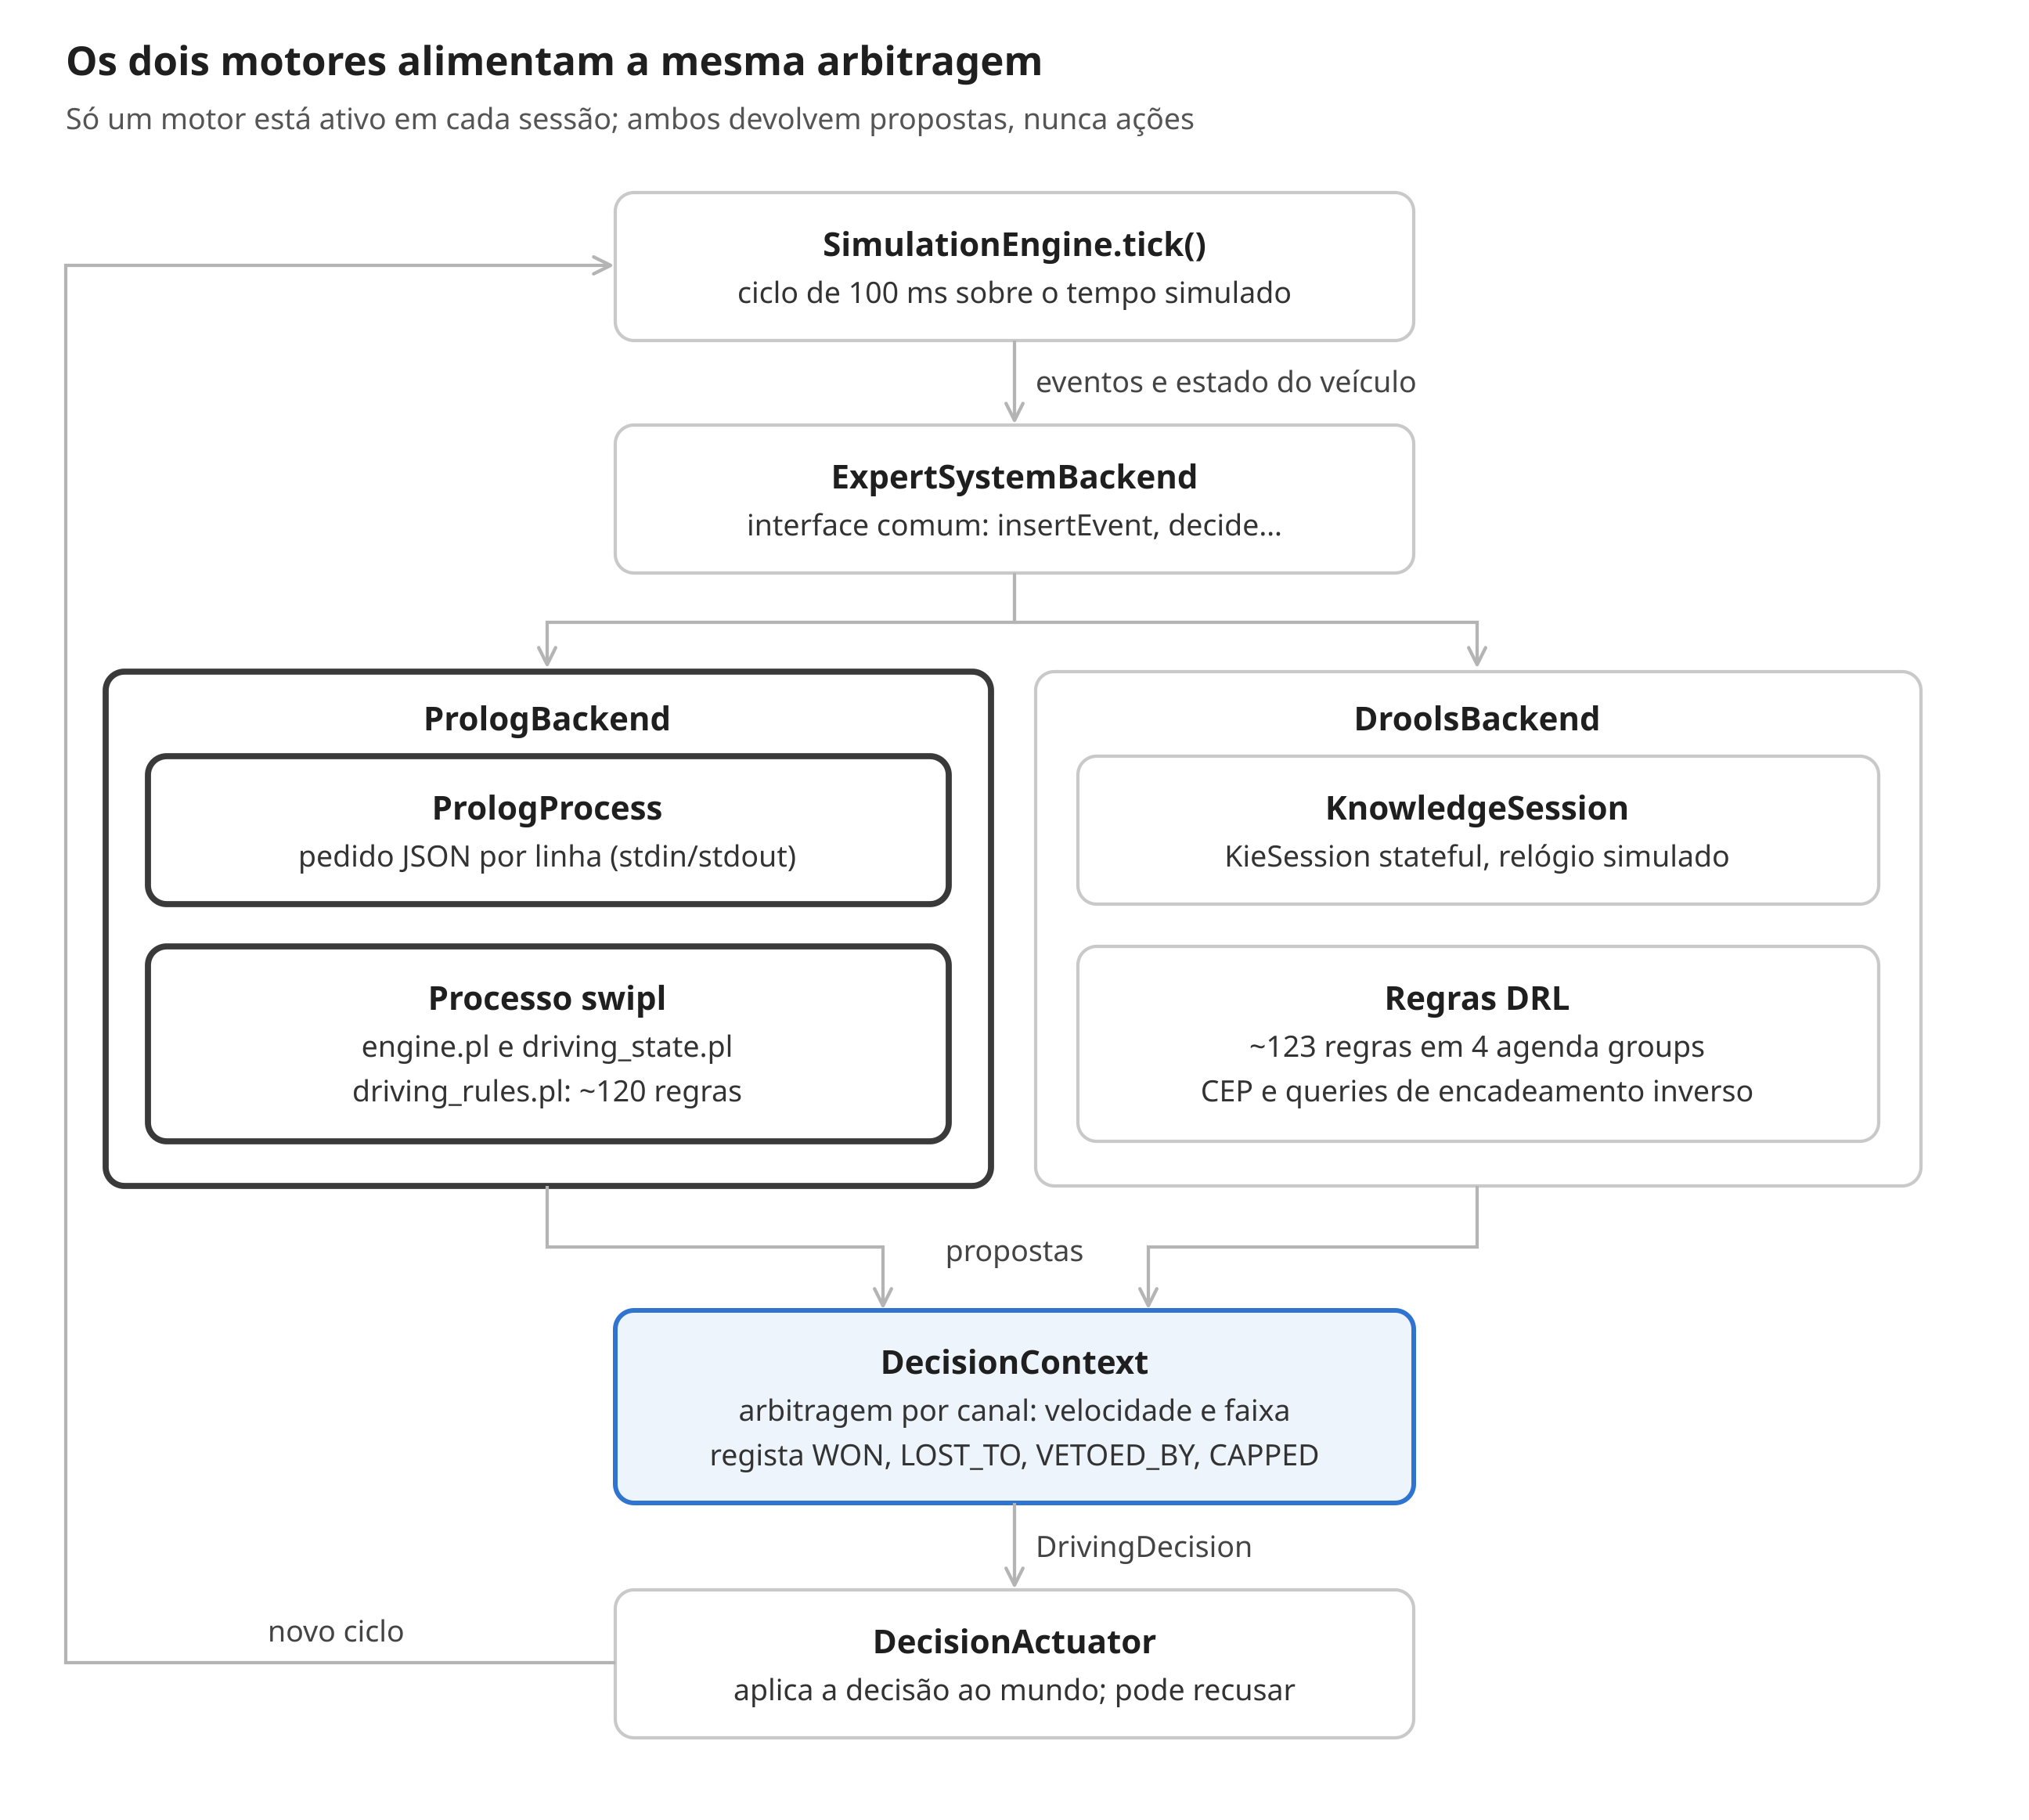
\includegraphics[width=0.78\textwidth]{figuras/arquitetura-motores.png}
  \caption{Os dois motores alimentam a mesma arbitragem: só um está ativo em
    cada sessão, e ambos devolvem propostas, nunca ações.}
  \label{fig:arquitetura-motores}
\end{figure}

\section{O motor de regras}
\label{sec:motor-regras}

As regras são dados: \texttt{rule(Id, Precedência, Condições, Ações)}. A
\cref{lst:regra-peao} mostra um exemplo.

\begin{lstlisting}[caption={Uma regra do motor Prolog (\texttt{driving\_rules.pl})},label=lst:regra-peao]
rule('Emergency stop for pedestrian extremely close',
     880,
     [ pedestrian_conflict(P),
       pedestrian(P, D),
       test(D =< 6.0) ],
     [ assert(proposal(emergency_brake, 0.0, critical, emergency_safety,
                       'Pedestrian critical distance in current path')) ]).
\end{lstlisting}

Uma condição pode ser um padrão a unificar com um facto, \cod{not(C)} (negação
por falha), \cod{test(Objetivo)} (aritmética ou um predicado auxiliar que lê os
factos através de \cod{known/1}) ou \cod{prove(Objetivo)}, provado por
encadeamento inverso (\cod{prove_goal/2}). A única ação é \cod{assert(Facto)}.
O motor faz assim encadeamento para a frente sobre os factos e encadeamento
inverso dentro das condições, por exemplo em \cod{safe_to_change_lane/1}, cujos
subobjetivos (\cod{maneuver_idle}, \cod{no_continuous_line}, \cod{side_clear},
\cod{room_to_follow}) descem até aos factos percebidos.

\begin{itemize}
  \item \textbf{Memória de trabalho:}
  \begin{itemize}
    \item \cod{wm_fact(Id, Facto)} guarda os factos do ciclo, tanto os
      percebidos como os derivados;
    \item \texttt{wm\_support(Id, Regra, Evidência)} guarda a justificação de cada
      facto derivado: a regra que o concluiu, os identificadores dos factos em
      que assentou e os padrões negados que se verificaram. Um facto sem
      suporte veio da perceção.
  \end{itemize}
  \item \textbf{Ciclo:} \cod{run_rules/0} avalia todas as regras e enche a
    agenda. Depois, até a agenda esvaziar, dispara a melhor ativação. A
    resolução de conflitos escolhe a maior precedência, depois a regra declarada
    primeiro e depois a correspondência encontrada primeiro. A refração impede
    que uma instanciação dispare duas vezes no mesmo ciclo. Os factos nunca são
    retirados dentro de um ciclo.
  \item \textbf{Estado entre ciclos:} fica em \cod{driving_state.pl}, o
    equivalente das 33 regras de perceção do Drools. Este ficheiro guarda as
    últimas leituras, a janela de TTC, o compromisso perante o semáforo, o
    cronómetro do STOP e o estado da ultrapassagem. No início de cada ciclo
    carrega tudo como factos (\cod{load_cycle_facts/0}). As regras não alteram
    estado: concluem o que mudou (por exemplo \cod{overtake_started/3}), e
    \cod{store_conclusions/0} grava-o no fim do ciclo.
\end{itemize}

\section{Comparação com o motor da unidade curricular}
\label{sec:comparacao-motor-uc}

O sistema não usa o motor da unidade curricular (\cod{sp_exp1.pl},
\cod{sp_exp2.pl}): o motor (\cod{engine.pl}) foi desenvolvido pelo grupo. O
problema exige decidir a cada 100\,ms sobre uma memória de trabalho que muda em
cada ciclo, disparar as regras pela mesma ordem que o Drools e devolver
explicações como dados ao Java, e não como texto na consola. Do motor da UC
manteve-se a ideia central: registar a justificação de cada facto quando é
concluído (\cod{justifica/3} corresponde ao nosso \cod{wm_support/3}) e
explicar a partir desse registo.

As regras do professor usam operadores e números
(\cod{regra 7 se [... e ...] entao [cria_facto(...)]}). As nossas são termos
simples, \texttt{rule(Id, Precedência, Condições, Ações)}, identificados pelo nome
da regra Drools que replicam e com uma precedência numérica. As condições do
professor são factos, \cod{nao} e \cod{avalia/1}, que compara um valor com uma
constante. As nossas acrescentam \cod{test/1}, com qualquer objetivo Prolog (por
exemplo, comparar a velocidade com o limite), e \cod{prove/1}, que prova o
objetivo por encadeamento inverso. O controlo também difere. O motor do
professor dispara uma regra assim que um facto a satisfaz. O nosso junta as
instanciações numa agenda, escolhe pela precedência e aplica refração.

A diferença principal está no metaconhecimento. No \cod{sp_exp2.pl},
\cod{facto_dispara_regras/2} indica que regras cada facto pode disparar, mas é
estático e escrito manualmente na base de conhecimento. Uma entrada em falta faz
com que a regra nunca seja tentada, sem qualquer erro. No nosso motor, o
metaconhecimento é dinâmico. \cod{ensure_index/0} deriva-o das próprias regras
quando o motor arranca, incluindo os factos lidos pelos predicados auxiliares, e
guarda-o em predicados dinâmicos (\cod{rule_reads/2}, \cod{rule_precedence/2},
\cod{rule_rank/2}). \cod{fired/2} muda a cada disparo. Nas explicações,
\cod{como/1} escreve na consola, enquanto \cod{explain/2} devolve a árvore de
derivação como termo. \cod{whynot/1} parte de um facto e desce recursivamente
pelas premissas, enquanto \cod{why_not/2} parte de uma regra e indica a condição
que a impediu de disparar. O motor do professor não tem explicação do tipo
\emph{Why}.
